\documentclass[11pt,a4paper]{article}
\usepackage[utf8]{inputenc}
\usepackage[T1]{fontenc}
\usepackage{lmodern}
\usepackage{amsmath,amssymb,amsfonts}
\usepackage{graphicx}
\usepackage{booktabs}
\usepackage{microtype}
\usepackage{hyperref}
\usepackage{url}
\usepackage{xcolor}
\usepackage{caption}
\usepackage{subcaption}
\usepackage{algorithm}
\usepackage{algpseudocode}
\usepackage{enumitem}
\usepackage{array}

\hypersetup{
    colorlinks=true,
    linkcolor=blue,
    citecolor=blue,
    urlcolor=blue,
    pdftitle={SCM: Sleep-Consolidated Memory for Language Agents},
    pdfauthor={SCM Research Team}
}

\title{SCM: Sleep-Consolidated Memory for Language Agents\\
\large An End-to-End, Reproducible Memory Lifecycle from Selective Encoding to Contradiction-Safe Consolidation}
\author{SCM Research Team}
\date{May 1, 2026}

\begin{document}
\maketitle

\begin{abstract}
Large language models are still weak at long-horizon memory management under interference, contradiction, and noise growth. Most deployed memory layers are either context-window extensions or append-only retrieval stores with limited lifecycle control. We present Sleep-Consolidated Memory (SCM), a full memory architecture that combines selective encoding, event-aware association binding, spreading-activation retrieval, staged sleep consolidation (MicroSleep and DeepSleep), adaptive forgetting dynamics, and contradiction-safe version lineage. Unlike isolated module proposals, SCM is implemented and evaluated as one integrated system across six development phases with artifact-backed benchmark suites. On the latest Phase 6 human-memory benchmark, SCM achieves one-shot recall accuracy 1.0000, MicroSleep disambiguation gain 1.0000, DeepSleep disambiguation gain 1.0000, deep-stage noise retention 0.0000, and contradiction-versioning accuracy 1.0000. In a 10-seed stress benchmark with 96 duplicate/noise pairs per seed, lexical retrieval, vector retrieval, and SCM awake-only remain at disambiguation recall 0.0000, while SCM+DeepSleep reaches mean disambiguation recall 0.9052 with mean noise retention 0.0000. In a seven-day long-horizon benchmark, sleep-enabled SCM reaches final family-aware disambiguation recall 0.9812 with final noise retention 0.0000, versus awake-only recall 0.0000 and noise retention 1.0000. A reproducibility pack reruns the full claim stack and reports overall pass. The resulting evidence supports SCM as a rigorous memory-lifecycle baseline for next-generation persistent language agents.
\end{abstract}

\section{Introduction}
Persistent memory remains a central bottleneck for language agents. Context-window approaches degrade when relevant information is not near prompt boundaries \cite{liu2023lost}. Retrieval-augmented systems improve factual access but often behave as growing stores with weak consolidation and weak forgetting control \cite{lewis2020retrieval}. System-style memory managers such as MemGPT improve scaling abstractions but are not, by construction, biologically grounded memory lifecycles \cite{packer2023memgpt}. Production memory layers such as Mem0 advance personalization but are still primarily awake-time retrieval systems \cite{chhikara2025mem0}.

Human memory is not append-only. It is selective at encoding, bounded in working capacity \cite{miller1956magical,baddeley1974working}, restructured by sleep \cite{rasch2013sleep}, and stabilized by active forgetting \cite{tononi2003sleep,sha2024forgetting}. This paper operationalizes those principles in a single architecture and evaluates whether sleep-centric lifecycle operations materially improve memory behavior under stress.

The central claim is specific: in controlled duplicate-pressure and long-horizon benchmarks, sleep-enabled SCM produces large disambiguation gains and strong noise suppression that do not appear in awake-only or standard retrieval controls.

\section{What This Project Built (A-Z)}
SCM was developed as a six-phase program, each phase shipping code, tests, and measurable artifacts.

\begin{table}[htbp]
\centering
\caption{Project build map from Phase 1 to Phase 6.}
\label{tab:phase_map}
\small
\begin{tabular}{>{\raggedright\arraybackslash}p{0.08\textwidth} >{\raggedright\arraybackslash}p{0.35\textwidth} >{\raggedright\arraybackslash}p{0.49\textwidth}}
\toprule
\textbf{Phase} & \textbf{Core capability} & \textbf{Evidence path} \\
\midrule
1 & Selective encoding, salience gating, grasp scoring, prediction-error signal & \url{src/core/attention_gate.py}; \url{tests/test_memory_pipeline.py} \\
2 & Event compiler and association binder with edge aging and pruning & \url{src/core/event_compiler.py}; \url{src/core/association_binder.py}; \url{research/metrics/phase6_guardrails_latest.json} \\
3 & Spreading activation retrieval and hypothesis ranking & \url{src/retrieval/spreading_activation.py}; \url{src/retrieval/hypothesis_ranker.py}; \url{tests/test_phase3_pipeline.py} \\
4 & MicroSleep and DeepSleep orchestration, replay, downscaling, synthesis & \url{src/sleep/micro_sleep.py}; \url{src/sleep/deep_sleep.py}; \url{tests/phase4_metrics.py} \\
5 & Adaptive forgetting dynamics and contradiction-safe version lineage & \url{src/sleep/forgetting_dynamics.py}; \url{src/core/long_term_memory.py}; \url{tests/test_contradiction_versioning.py} \\
6 & Guardrails, human-memory suite, baseline comparison, long horizon, reproducibility pack & \url{research/metrics/phase6_human_memory_latest.json}; \url{research/metrics/baseline_comparison_latest.json}; \url{research/reproducibility/reproducibility_pack_latest.json} \\
\bottomrule
\end{tabular}
\normalsize
\end{table}

This paper describes the integrated system, not a single module in isolation.

\section{System Architecture}
\subsection{Memory Substrates}
SCM uses a bounded working memory plus persistent graph long-term memory:
\begin{itemize}[leftmargin=1.4em]
    \item \textbf{Working memory:} capacity-constrained episodic buffer (default capacity 7).
    \item \textbf{Long-term memory:} typed concept graph with weighted relations, persistence, and version lineage metadata.
\end{itemize}

\begin{figure}[htbp]
\centering
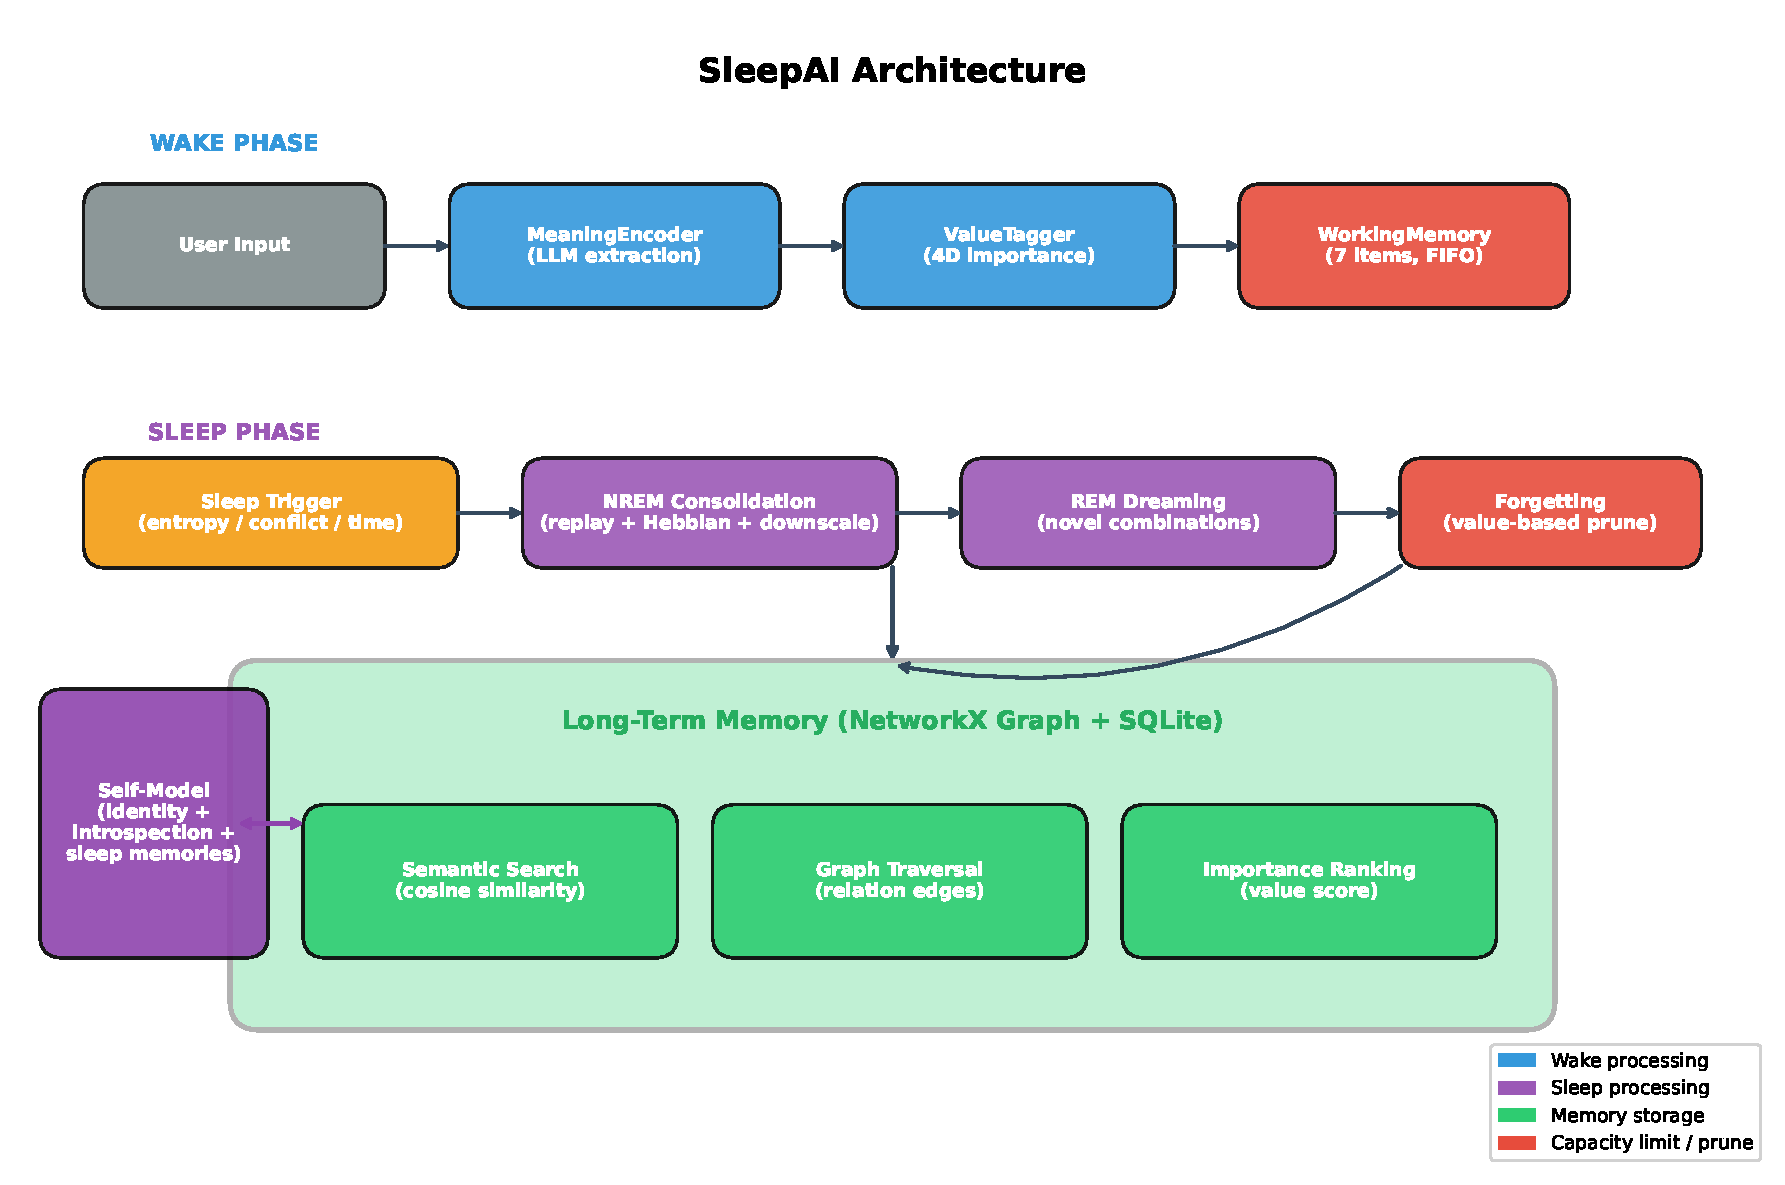
\includegraphics[width=0.95\textwidth]{figures/architecture.pdf}
\caption{SCM architecture: selective encoding and event binding during wake, staged consolidation and forgetting during sleep, and contradiction-safe version lineage across updates.}
\label{fig:architecture}
\end{figure}

\subsection{Sleep-State Control}
Sleep mode selection is pressure-aware:
\begin{itemize}[leftmargin=1.4em]
    \item MicroSleep trigger examples: entropy spike, turn interval, conflict pressure.
    \item DeepSleep trigger examples: high pressure, idle-time window, long session threshold.
\end{itemize}

\begin{figure}[htbp]
\centering
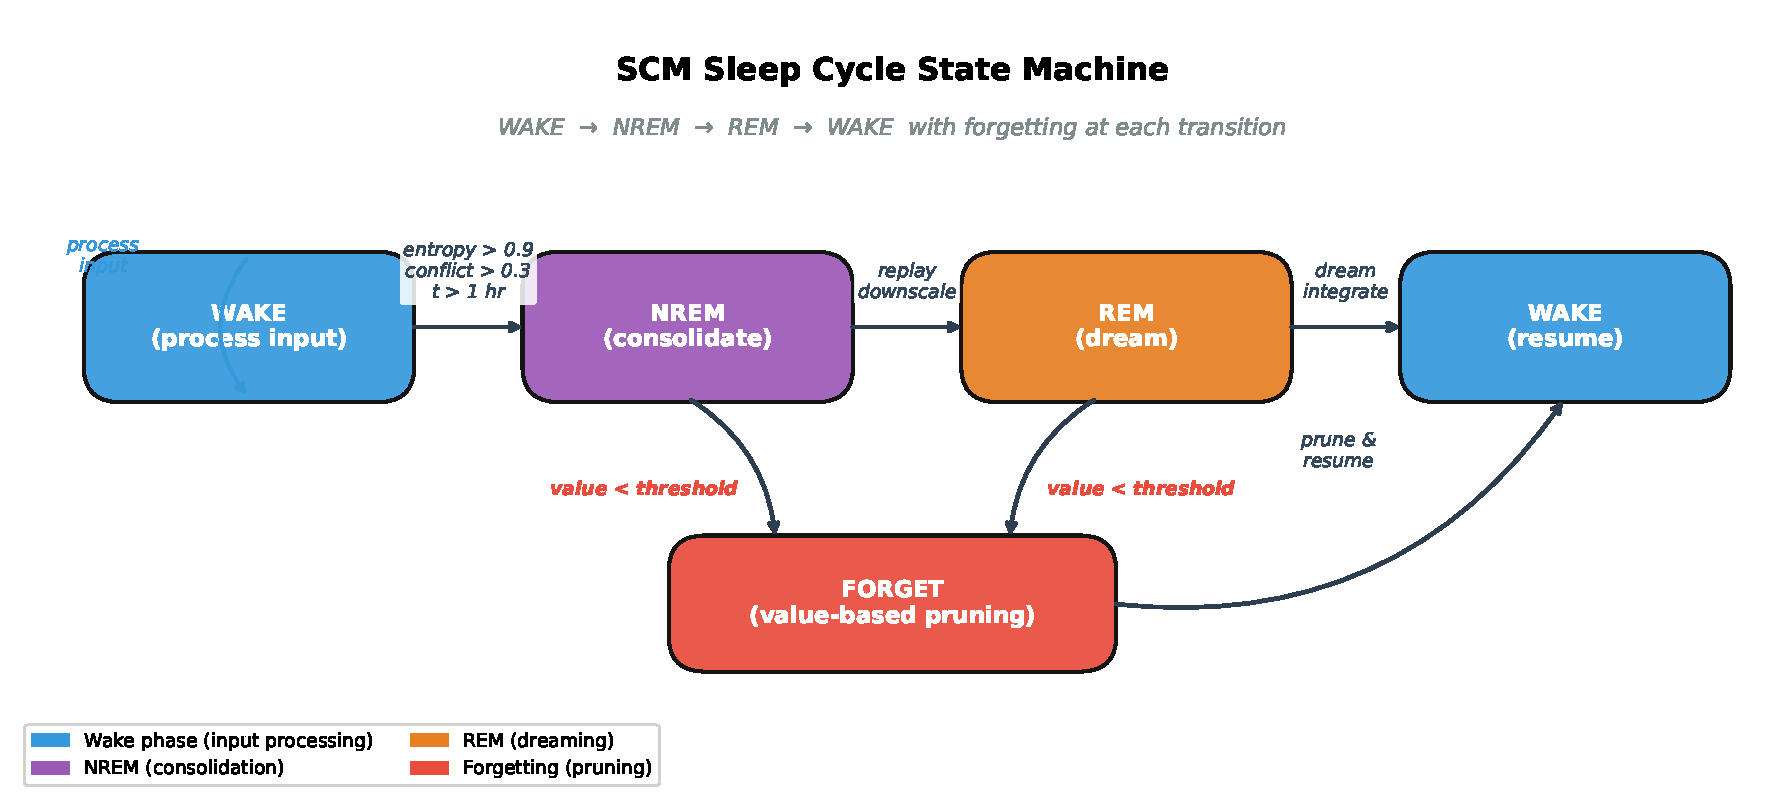
\includegraphics[width=0.85\textwidth]{figures/sleep_state_machine.pdf}
\caption{Wake/MicroSleep/DeepSleep control flow used by the orchestrator.}
\label{fig:sleep_state_machine}
\end{figure}

\section{Mathematical Formulation of SCM}
\subsection{Phase 1: Selective Encoding and Grasp}
For an input trace $x$, SCM computes adjusted salience
\begin{equation}
S_{\text{att}}(x) = \mathrm{clip}\left(
w_n N + w_t T + w_e |E| + w_r R + w_p \varepsilon - P_{\text{noise}},\ 0,\ 1
\right),
\label{eq:salience}
\end{equation}
where $N, T, E, R, \varepsilon$ are novelty, task relevance, emotional valence, repetition, and prediction error signals. In the current default configuration,
\[
(w_n, w_t, w_e, w_r, w_p) = (0.30, 0.35, 0.15, 0.10, 0.10).
\]

One-shot grasp is then estimated as
\begin{equation}
G(x) = \mathrm{clip}\left(
\alpha S_{\text{att}} + \beta O_{\text{schema}} + \gamma C_{\text{clarity}} - \delta L_{\text{load}},\ 0,\ 1
\right),
\label{eq:grasp}
\end{equation}
with $(\alpha,\beta,\gamma,\delta)=(0.40,0.30,0.20,0.10)$.

\subsection{Phase 2: Event-Aware Association Binding}
Given concepts $c_i,c_j$ in an event, relation strength increment is
\begin{equation}
\Delta w_{ij} = \eta \cdot \frac{g_i + g_j}{2} \cdot s_{\text{event}} \cdot q_{ij},
\label{eq:assoc_delta}
\end{equation}
with learning rate $\eta=0.30$ and
\begin{equation}
q_{ij} = \mathrm{clip}\left(0.45 \, s_{ij}^{\text{sem}} + 0.25 \, s_{ij}^{\text{tok}} + 0.30 \, s_{ij}^{\text{ctx}},\ 0.05,\ 1.0\right).
\label{eq:assoc_signal}
\end{equation}
Edges are aged by repeated multiplicative decay and pruned when stale and weak.

\subsection{Phase 3: Spreading Activation Retrieval}
SCM retrieval is cue-seeded graph propagation:
\begin{equation}
A_j^{(t+1)} = \delta A_j^{(t)} + \sum_{i} A_i^{(t)} W_{ij}\Gamma_{ij},
\label{eq:spreading}
\end{equation}
where $\delta=0.45$ is spreading decay, $W_{ij}$ relation strength, and $\Gamma_{ij}$ context gate.

The gate incorporates session/person matches and recency:
\begin{equation}
\Gamma = \mathrm{clip}\left(k_{\text{session}} \cdot k_{\text{person}} \cdot (0.6+0.4 r_{\text{recency}}),\ 0.3,\ 1.5\right).
\label{eq:context_gate}
\end{equation}

Candidate ranking blends cue match and consolidation score, and a recency-boosted variant is used in dedicated retrieval paths.

\subsection{Phase 4: Sleep Consolidation}
\textbf{MicroSleep.} Concept instability is
\begin{equation}
u(c)=0.40(1-r_c)+0.30e_c+0.20n_c+0.10(1-\tilde{s}_c),
\label{eq:instability}
\end{equation}
where $r_c$ is retention, $e_c$ prediction error, $n_c$ novelty, and $\tilde{s}_c$ normalized strength. Top-$k$ unstable traces are replayed and lightly reinforced; near-duplicate traces are merged.

\textbf{DeepSleep.} NREM performs Hebbian strengthening and downscaling; REM optionally synthesizes new links; forgetting then retires weak traces. A global downscale factor (default 0.90) is applied to concept and relation strengths.

\subsection{Phase 5: Forgetting Dynamics and Versioning}
Retention score follows
\begin{equation}
R(c)=p_1 G_c + p_2 S_c + p_3 H_c + p_4 D_c + p_5 \mathrm{Rec}_c - p_6 I_c,
\label{eq:retention}
\end{equation}
with default
\[
(p_1,p_2,p_3,p_4,p_5,p_6)=(0.22,0.24,0.18,0.18,0.12,0.22).
\]

Trace-specific decay is
\begin{equation}
\lambda_c=\lambda_0\left(1+1.5(1-R(c))+0.8I_c+\pi_{\text{version}}+\pi_{\text{state}}\right),
\label{eq:decay}
\end{equation}
with $\lambda_0=0.04$, then
\begin{equation}
s_c \leftarrow \max\left(0.05,\ s_c \exp\left(-\lambda_c \max(0.25,\mathrm{age\_hours}/24)\right)\right).
\label{eq:strength_decay}
\end{equation}

Adaptive thresholding increases forgetting pressure with memory load:
\begin{equation}
\theta_f=\min\left(0.85,\ \theta_s + 0.18\min(1,|M|/100) + 0.05\rho\right).
\label{eq:adaptive_threshold}
\end{equation}

Contradiction updates use version matching by similarity-plus-context scoring. If score exceeds threshold (default 0.70), the previous concept is archived and linked as a contradiction edge to the new active version.

\section{Experimental Design}
\subsection{Artifact-Centric Protocol}
All claims in this paper are tied to current machine-readable artifacts:
\begin{itemize}[leftmargin=1.4em]
    \item \url{research/metrics/phase6_human_memory_latest.json}
    \item \url{research/metrics/baseline_comparison_latest.json}
    \item \url{research/metrics/long_horizon_latest.json}
    \item \url{research/metrics/phase6_guardrails_latest.json}
    \item \url{research/metrics/phase6_backend_smoke_latest.json}
    \item \url{research/reproducibility/reproducibility_pack_latest.json}
\end{itemize}

\subsection{Benchmarks}
\textbf{Human-memory suite.} One-shot recall, sleep gain, selective forgetting, contradiction versioning.

\textbf{Baseline stress comparison.} 10 seeds (7001--7010), 96 duplicate/noise pairs per seed. Controls: lexical retrieval, vector retrieval, SCM awake-only baseline, SCM+MicroSleep, SCM+DeepSleep.

\textbf{Long-horizon benchmark.} Seven-day synthetic memory history with repeated interference, extra noise injection, periodic deep sleep, and late contradiction update.

\textbf{Guardrails and smoke.} Phase 2/4/6 status checks, deprecation scan, regression pytest bundle, backend endpoint smoke.

\section{Results}
\subsection{Core Human-Memory Behavior}
\begin{table}[htbp]
\centering
\caption{Phase 6 human-memory benchmark (latest artifact).}
\label{tab:phase6_core}
\begin{tabular}{@{}lc@{}}
\toprule
\textbf{Metric} & \textbf{Value} \\
\midrule
One-shot recall accuracy & 1.0000 \\
MicroSleep disambiguation gain (absolute) & 1.0000 \\
DeepSleep disambiguation gain (absolute) & 1.0000 \\
DeepSleep noise retention & 0.0000 \\
Contradiction-versioning accuracy & 1.0000 \\
Overall status & pass \\
\bottomrule
\end{tabular}
\end{table}

\begin{figure}[htbp]
\centering
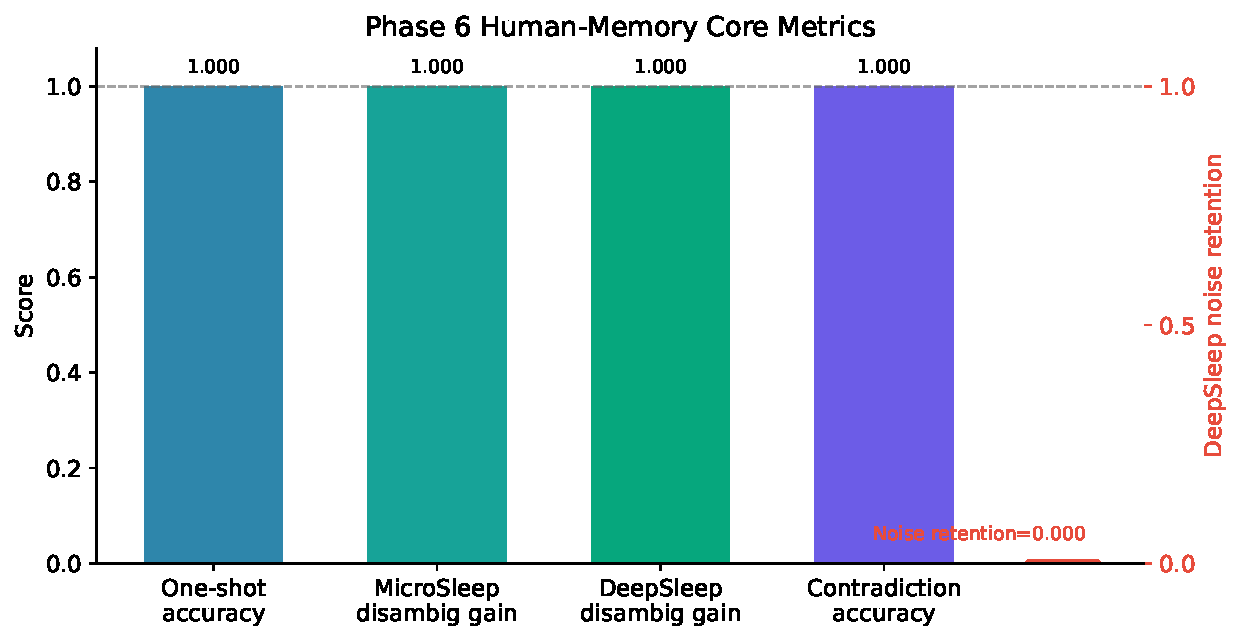
\includegraphics[width=0.90\textwidth]{figures/phase6_core_metrics.pdf}
\caption{Phase 6 core metrics from the latest human-memory artifact.}
\label{fig:phase6_core}
\end{figure}

\subsection{Stress Comparison Against Controls}
\begin{table}[htbp]
\centering
\caption{Baseline stress comparison (10 seeds, 96 pairs per seed).}
\label{tab:baseline}
\begin{tabular}{@{}lccc@{}}
\toprule
\textbf{Method} & \textbf{Disambiguation recall} & \textbf{Noise retention} & \textbf{Latency (ms)} \\
\midrule
Lexical retrieval baseline & 0.0000 & 1.0000 & 0.5394 \\
Vector retrieval baseline & 0.0000 & 1.0000 & 15.4428 \\
SCM baseline (no sleep) & 0.0000 & 1.0000 & 1.9302 \\
SCM + MicroSleep & 1.0000 & 0.0000 & 1.4698 \\
SCM + DeepSleep & 0.9052 & 0.0000 & 31.1439 \\
\bottomrule
\end{tabular}
\end{table}

\begin{figure}[htbp]
\centering
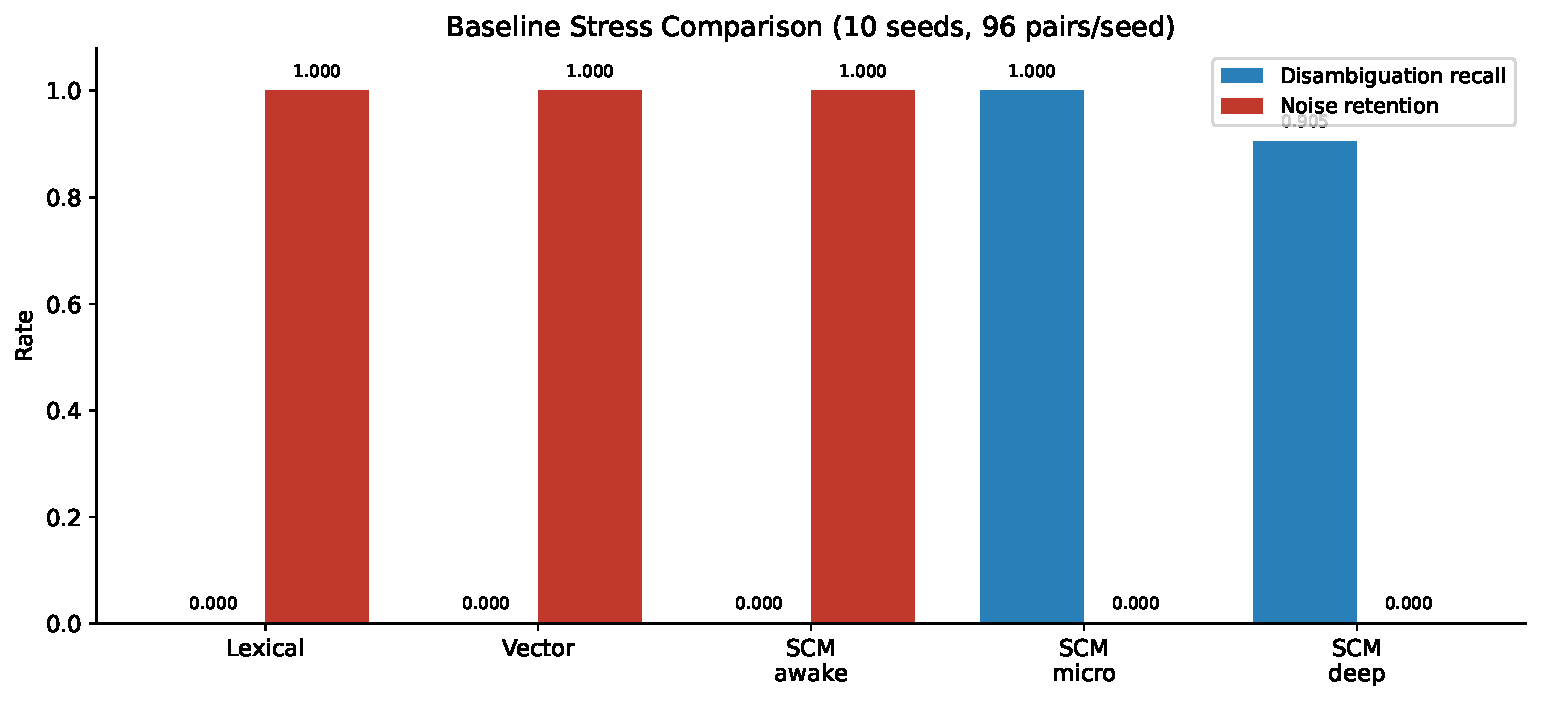
\includegraphics[width=0.95\textwidth]{figures/baseline_behavior_comparison.pdf}
\caption{Disambiguation vs. noise-retention behavior across controls and sleep-enabled SCM variants.}
\label{fig:baseline_behavior}
\end{figure}

The attribution signal is sharp: in this stress setting, all awake controls remain at 0.0000 disambiguation recall, while both sleep-enabled variants move to high-recall/low-noise regimes.

\subsection{Long-Horizon Memory}
\begin{table}[htbp]
\centering
\caption{Final-day long-horizon comparison (day 7).}
\label{tab:long_horizon}
\begin{tabular}{@{}lcc@{}}
\toprule
\textbf{Metric} & \textbf{Awake-only} & \textbf{Sleep-enabled} \\
\midrule
Family-aware disambiguation recall & 0.0000 & 0.9812 \\
Strict disambiguation recall & 0.0000 & 0.0000 \\
Noise retention & 1.0000 & 0.0000 \\
Anchor hit rate & 1.0000 & 1.0000 \\
\bottomrule
\end{tabular}
\end{table}

\begin{figure}[htbp]
\centering
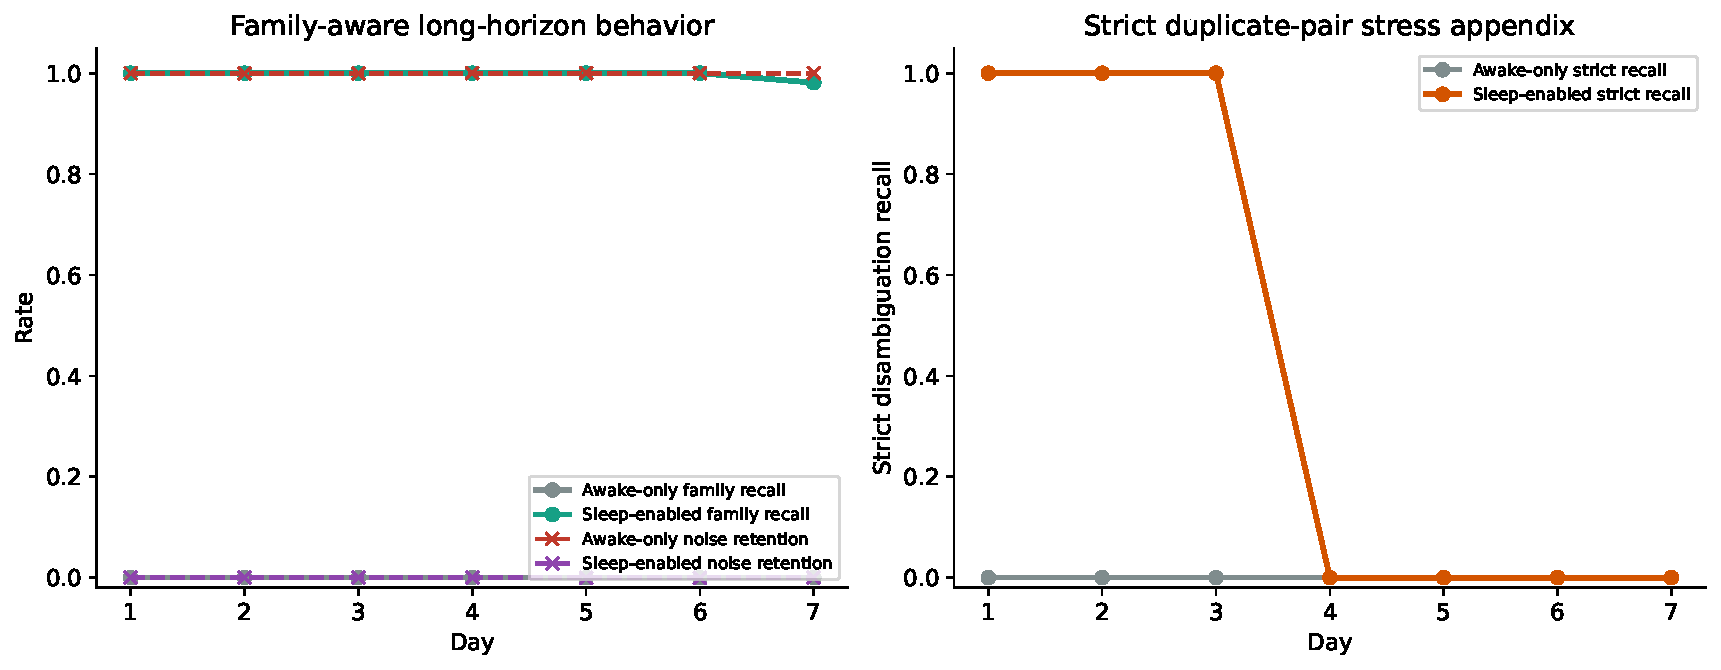
\includegraphics[width=0.98\textwidth]{figures/long_horizon_curves.pdf}
\caption{Long-horizon daily curves: family-aware release metric and strict duplicate-pair stress appendix.}
\label{fig:long_horizon}
\end{figure}

Family-aware duplicate recall is the release gate in the current benchmark design, while strict duplicate-pair recall is preserved as a transparent stress appendix.

\subsection{Reliability and Reproducibility}
Guardrail status reports pass across Phase 2, Phase 4, and human-memory checks, with zero hits for tracked deprecation patterns. Backend smoke reports 20/20 HTTP success, 20/20 overall pass, mean latency 45.2 ms, p50 22.7 ms, and p90 26.3 ms.

The reproducibility pack reruns baseline comparison, long-horizon benchmark, Phase 6 guardrails, and a smoke pytest bundle in one command chain, reporting overall pass and logging artifact fingerprints.

\begin{table}[htbp]
\centering
\caption{Reproducibility pack execution summary (latest run).}
\label{tab:repro}
\begin{tabular}{@{}lcc@{}}
\toprule
\textbf{Suite} & \textbf{Result} & \textbf{Duration (ms)} \\
\midrule
baseline\_comparison & pass & 58443.53 \\
long\_horizon & pass & 7296.59 \\
phase6\_guardrails & pass & 21499.70 \\
smoke\_pytests & pass & 7291.73 \\
\bottomrule
\end{tabular}
\end{table}

\section{Why the Gains Appear}
The combined evidence supports a mechanism-level interpretation.
\begin{enumerate}[leftmargin=1.4em]
    \item \textbf{Selective encoding} reduces early contamination from weak traces.
    \item \textbf{Association binding} creates retrievable structure beyond pure embedding similarity.
    \item \textbf{Sleep consolidation} reshapes graph topology and strength distributions.
    \item \textbf{Adaptive forgetting} prunes low-value distractors and preserves strong traces.
    \item \textbf{Version lineage} prevents contradiction updates from destructive overwrite.
\end{enumerate}

The strongest empirical support for this interpretation is negative evidence from controls: lexical, vector, and awake-only SCM stay at 0.0000 disambiguation recall in the 96-pair stress setting.

\section{Limitations and Claim Boundaries}
This work is strong on internal reproducibility, but still has clear boundaries.
\begin{itemize}[leftmargin=1.4em]
    \item Benchmarks are mostly synthetic and harness-driven.
    \item External head-to-head comparisons remain limited.
    \item Strict duplicate-pair disambiguation under long horizons remains a known stress weakness.
    \item Claims are about human-like memory dynamics, not consciousness or sentience.
\end{itemize}

Accordingly, the strongest defensible claim today is not ``human equivalence,'' but that a sleep-consolidated lifecycle can outperform awake-only memory pipelines on targeted memory-quality criteria with reproducible evidence.

\section{Conclusion}
SCM demonstrates that memory quality for language agents improves when memory is treated as a lifecycle rather than as static retrieval storage. Across Phase 6 artifacts, SCM preserves one-shot behavior, executes contradiction-safe updates, suppresses low-value noise, and delivers large disambiguation gains in pressure settings where awake controls fail. The next research milestone is external user validation at scale with broader cross-system baselines.

\section*{Reproducibility Statement}
Core reproducibility entry points:
\begin{itemize}[leftmargin=1.4em]
    \item \url{tests/baseline_comparison.py}
    \item \url{tests/long_horizon_benchmark.py}
    \item \url{tests/phase6_guardrails.py}
    \item \url{tests/reproducibility_pack.py}
\end{itemize}
Latest aggregate evidence:
\begin{itemize}[leftmargin=1.4em]
    \item \url{research/reproducibility/reproducibility_pack_latest.json}
    \item \url{docs/SCM_REPRODUCIBILITY_PACK.md}
\end{itemize}

\appendix
\section{High-Level Sleep Orchestration}
\begin{algorithm}[htbp]
\caption{SCM Sleep Orchestration (simplified)}
\label{alg:sleep}
\begin{algorithmic}[1]
\Require Concepts $C$, Relations $R$, Episodes $E$
\If{DeepSleep trigger}
    \State $(C',R') \gets \text{NREM\_consolidate}(C,R,E)$
    \State $(C'',R'') \gets \text{REM\_synthesize}(C',R')$
    \State $(C^*,R^*) \gets \text{ForgettingDynamics}(C'',R'')$
\ElsIf{MicroSleep trigger}
    \State $(C^*,R^*) \gets \text{MicroSleep}(C,R,E)$
\Else
    \State $(C^*,R^*) \gets (C,R)$
\EndIf
\State \Return $(C^*,R^*)$
\end{algorithmic}
\end{algorithm}

\section{Contradiction-Safe Versioning Logic}
When a new concept $c_{\text{new}}$ is added with versioning enabled, SCM searches for a type-matched candidate $c_{\text{old}}$ using similarity plus context bonuses. If the score exceeds threshold:
\begin{enumerate}[leftmargin=1.4em]
    \item mark $c_{\text{old}}$ as archived and no longer current;
    \item set $c_{\text{new}}.\text{version\_parent}=c_{\text{old}}$ and inherit root lineage;
    \item insert a directed contradiction relation $c_{\text{old}} \rightarrow c_{\text{new}}$;
    \item keep retrieval on current versions by default, while preserving history for audit.
\end{enumerate}

\bibliographystyle{plain}
\bibliography{references}

\end{document}
